\noindent \textit{Peskin and Schroeder}, page 294 \\

\noindent Recall the classical Lagrangian density $\mathcal{L} = \bar{\psi}(i \slashed{D} - m) \psi - \frac{1}{4} F_{\mu\nu}^{\,\,\,\,a} F^{\mu\nu, \, a}$, where $a$ denotes individual fields, that we crafted to be invariant under the local gauge symmetry group $SU(2)$. We introduced the ``helper'' gauge field $A_{\mu}^a$ which manifests in the terms of the spacetime curvature tensor , or the curvature of the $SU(2)$ fibre bundle, $F_{\mu\nu} = -i [D_\mu, D_\nu]$, where $D_\mu = \partial_\mu - i g A_\mu^a \frac{\sigma^a}{2}$ is the covariant derivative. \\

\noindent This Langrangian density represents a nontrivial dynamical system that is invariant under the local gauge symmetry group and endows fermions, as well as other fields, with dynamics. Unlike many other effective classical theories, this one is not quadratic in its fields and yields nonlinear equations of motion (e.g., instanton and soliton solutions). \\

\noindent We now quantize this gauge theoryto build a quantum theory that is invariant under the Poincar\'e and local gauge symmetry groups by finding the correct representation that has this Lagrangian density as its effective classical limit. \\

\noindent Two problems that arise for the gauge theories are (1) the classical theory ($\mathcal{L}_0$) is already nonlinear, and (2) there are lots of symmetries, global and local. Local symmetries are represented by copies of $SU(2)$ acting independently of each other at each spacetime location. \\

\noindent Two approaches of quantization that we will explore include (1) an analytic, but naive \textit{path integral quantization} $\int \mathcal{D} A \mathcal{D} \psi \mathcal{D} \bar{\psi} e^{i S}$ that is good for high-energy scattering processes, but not for calculating ground state correlation functions. The mathematical rigor of this approach is a current topic of research. And (2) a computational route of \textit{lattice quantization}, which makes dealing with nonlinearity ``easy'', but it loses Poincar\'e invariance in the process. Note that there is also the route of canonical quantization, but we will not bother with that here.

\subsection*{Path Integral Quantization of Gauge Theories}

\noindent First, some words on the space of all gauge fields $A_\mu^a$: note that $A_\mu^a \frac{\sigma^a}{2}$ and $A_\mu^a \frac{\sigma^a}{2} + \frac{1}{g} (\partial_\mu \alpha^a) \frac{\sigma^a}{2} + i [\alpha^b \frac{\sigma^b}{2}, \alpha^c \frac{\sigma^c}{2}]$ are \textit{gauge equivalent}, meaning that there exists an infinite number of $A_\mu^a$'s with the same path integrand $e^{i S}$, causing the path integral to result in infinity, since we are redundantly integrating over a continuous infinity of physically equivalent field configurations. \\

\noindent Consider the gauge field $A_\mu^a$, a list of 12 numbers in $(3+1)$-dimensional spacetime, on $(0+1)$-dimensional spacetime $\mathcal{M}_{0+1}$ (e.g., a line), where $A_\mu^a$ is still a list of three numbers. Now, $SU(2)$ acts independently on $A_\mu^a$ at each point in $\mathcal{M}_{0+1}$. This action is tantamount to multiplying by a phase on a sphere $S^3$ at each spacetime location, since $SU(2)$ is parameterized by four numbers, the coefficients of the quaternions with norm equal to one. Below is a schematic of the space of all $A_\mu^a$'s. \\

\begin{figure}[H]
	\centering
	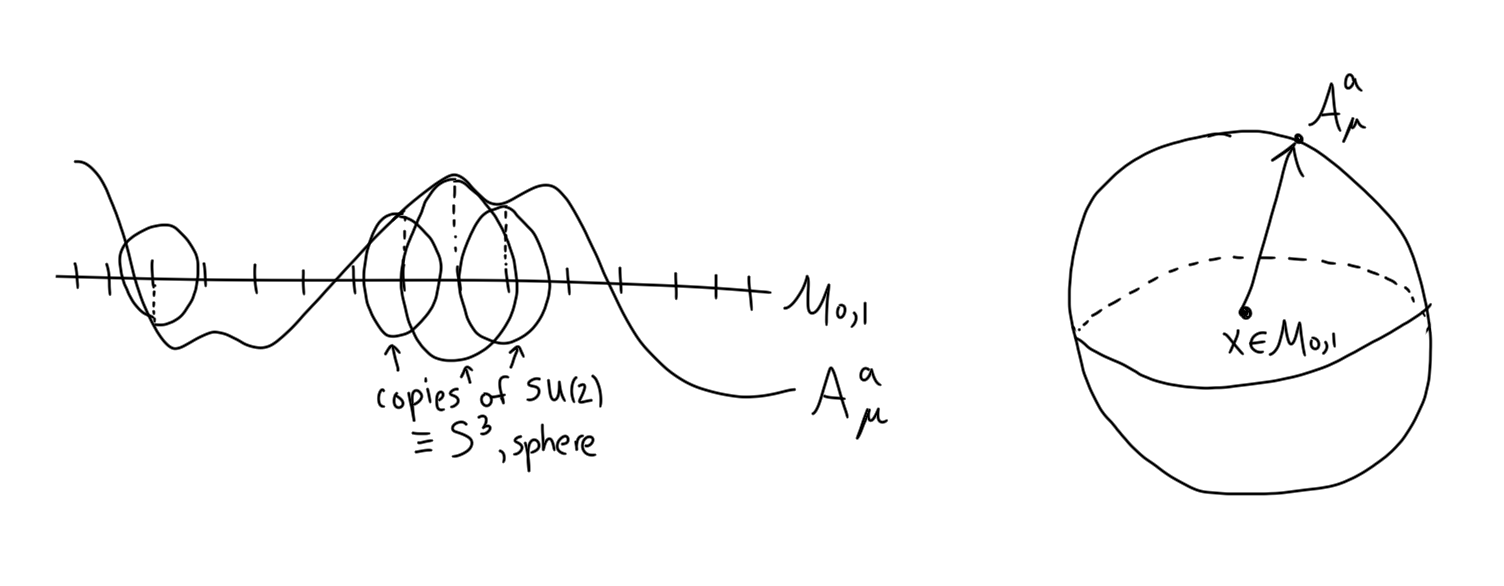
\includegraphics[width=4in]{images/su2schematic.png}
	\caption*{Schematic of gauge field configurations, independent copies of $SU(2)$ acting on $(0+1)$-dimensional spacetime.}
\end{figure}

\noindent So $A_\mu^a$ is like a vector on $S^3$ at each spacetime location and is a possible configuration in $\mathcal{M}_{0+1}$. These configurations form an equivalence class  $[A_\mu^a]$ defined by the local gauge group $\mathcal{G}$. Addressing the problem of very many symmetries, global and local,  in the path integral approach, there are very many equivalence classes, or configurations, to sum over, but we'd like to just choose one configuration. \\

\noindent Another, more common schematic to demonstrate the action of gauge groups is to consider rotations in $SO(2)$, where our theory is a zero-dimensional theory invariant under $SO(2)$. Configurations in this schematic are just points in a two-dimensional space with equivalence classes defined by circles centered at the origin. See schematic below. \\

\begin{figure}[H]
	\centering
	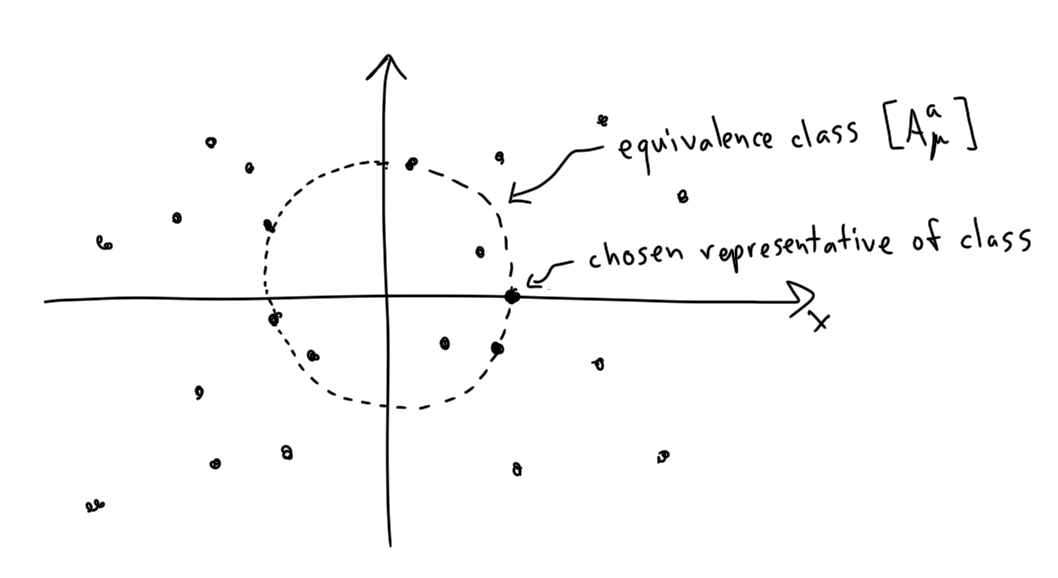
\includegraphics[width=4in]{images/so2schematic.png}
	\caption*{Schematic of gauge field configurations and equivalence classes represented by rotations in $SO(2)$.}
\end{figure}

\noindent In choosing a representative point per equivalence class, we enforce the \textit{gauge fixing condition}. A good choice of representative may be the point that crosses the horizontal axis. We then integrate over the space of the chosen representatives. This effectively reduces the size of the configuration space and makes the path integral much more tractable. \\

\noindent Note that we only pick one representative per equivalence class, but there can be more than one depending on the choice of gauge fixing condition, where the gauge fixing condition if a function that crosses the equivalence class circle more than once. This is called the \textit{Gribov ambiguity}, and commonly happens in the Coulomb gauge. \\

\begin{figure}[H]
	\centering
	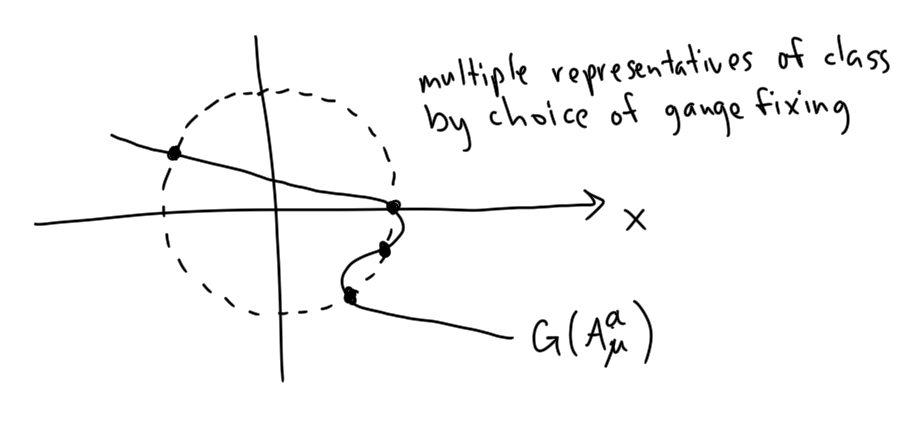
\includegraphics[width=3in]{images/gribov.png}
	\caption*{Example schematic of Gribov ambiguity, where more than one representative of the equialvence class is chosen by the guage fixing condition.}
\end{figure}

\subsubsection*{Gauge Fixing Condition}

\noindent Recall that the path integral approach is made difficult by the fact that we are redundantly integrating over a continuous infinity of physically equivalent field configurations. By applying a gauge fixing condition, we isolate the intersting part of the integral and count each distinct physical configuration only once. Finding the right gauge fixing function $G$ allows us to separate out this overcounting in the path integral and throw it away. Note that we are free to ``throw it away'' since we are \textit{guessing} a quantum theory.\\

\noindent Choosing the gauge fixing function to be $G(A_\mu^a) = \partial_\mu A_\mu^a - \omega^a$, where $\omega^a$ is any scalar field, is a generalization of the Lorentz gauge, and setting this equal to zero is a generalization of the Lorentz gauge condition

\begin{equation}
G(A_\mu^a) = \partial_\mu A_\mu^a - \omega^a = 0.
\end{equation}

\noindent With the gauge fixing function, the way we separate the overcounting is by inserting unity

\begin{equation}
1 = \int \mathcal{D} \alpha \,\, \delta(G(A^\alpha)) \, \text{det} \left( \frac{\delta G(A^\alpha)}{\delta \alpha} \right).
\end{equation}

\noindent Breaking equation this down, we are performing a path integral over all possible gauge transformations, and picking out only the $G(A^\alpha)$ that equals zero, obeying the gauge fixing condition, choosing a single representative of the equivalence class. The determinant is called the \textit{Faddeev-Popov determinant}. The notation $A^\alpha$ indicates the locally gauge transformed gauge field

\begin{align}
(A^\alpha)^a_\mu &= A^a_\mu + \frac{1}{2} \partial_\mu \alpha^a + f^{abc} A_\mu^b \alpha^c \\
&= A_\mu^a + \frac{1}{g} D_\mu \alpha^a
\end{align}

\noindent Where $f^{abc}$ are the structure constants from the Pauli spin matrix commutation relations

\begin{equation}
\left[ \frac{\sigma^a}{2}, \frac{\sigma^b}{2} \right] = i f^{abc} \frac{\sigma^c}{2}.
\end{equation}

\noindent This way of writing 1 is the continuous, functional generalization of that for discrete, many-variable $n$-dimensional vectors

\begin{equation}
1 = \left( \prod_{j=1}^n \int d a_j \right) \delta^{(n)} (\textbf{g}(\textbf{a})) \text{det} \left( \frac{\partial g_j}{\partial a_k} \right)
\end{equation}

\noindent Where the determinant here is the Jacobian of the change of variables. By change of variables, this can be written as (\textbf{Exercise})

\begin{equation}
1 = \left( \prod_{j=1}^n \int d b_j \right) \delta^{(n)} (\textbf{b}).
\end{equation}

\noindent Inserting the contiuous, functional version of one into the path integral, we now have an expression that integrates over the equivalence classes but ``sucks out'' the overcounting to just one representative of the class

\begin{equation}
\int \mathcal{D} \alpha \int \mathcal{D} A \mathcal{D} \psi \mathcal{D} \bar{\psi} \,\, \delta(G(A^\alpha)) \text{det} \left( \frac{\delta G(A^\alpha)}{\delta \alpha} \right) e^{i S}.
\end{equation}

\noindent Evaluating the Faddeev-Popov determinant in our choice of the Lorentz gauge (\textbf{Exercise})

\begin{align}
\text{det} \left( \frac{\delta G(A^\alpha)}{\delta \alpha} \right) &= \text{det} \left( \frac{1}{g} \partial^\mu D_\mu \right) \\
&= \int \mathcal{D} c \mathcal{D} \bar{c} \,\, e^{i \frac{1}{g} \int d^4 x \, \bar{c} (-\partial^\mu D_\mu) c}
\end{align}

\noindent Where, recall from the study of fermions, we have used auxiliary Grassman-valued, scalar, spin-0 fields $c$ and $\bar{c}$. These fields are non-physical and must disappear form the final results: \textit{Faddeev-Popov ghosts} or \textit{ghosts}. \\

\noindent Inserting the ghost expression for the determinant into the path integral, we now have

\begin{align}
\int \mathcal{D} \alpha \int \mathcal{D} A \int \mathcal{D} c \mathcal{D} \bar{c} \int \mathcal{D} \psi \mathcal{D} \bar{\psi} \,\, \delta( \partial^\mu A^a_\mu - \omega^a ) e^{i (S + \frac{1}{g} \int d^4 x \, \bar{c} (-\partial^\mu D_\mu) c)}.
\end{align}

\noindent Integrate out the delta functional, since $\omega^a$ is arbitrary, using an Gaussian integral over $\omega^a$ with coefficient $\xi \in [0,1]$, and calling $S' = S + \frac{1}{g} \int d^4 x \, \bar{c} (-\partial^\mu D_\mu) c$,

\begin{equation}
\int \mathcal{D} \omega \, e^{-i \int d^4 x \, \frac{1}{2} \xi (\omega^a)^2} \left( \int \mathcal{D} ... \right) \delta( \partial^\mu A_\mu^a - \omega^a) e^{i S'}
\end{equation}

\noindent Since $\omega^a$ is an arbitrary, gauge-fixing, scalar function that takes one representative of each independent equivalence class, the full path integral will now be independent of $\omega^a$, and we have the form

\begin{equation}
N(\xi) \int \mathcal{D} \alpha \int \mathcal{D} A \int \mathcal{D} c \mathcal{D} \bar{c} \int \mathcal{D} \psi \mathcal{D} \bar{\psi} \,\,  e^{i \int d^4 x \, \mathcal{L}'} .
\end{equation}

\noindent The Lagrangian $\mathcal{L}'$ has the form

\begin{equation}
\mathcal{L}' = \bar{\psi} (i \slashed{D} - m) \psi - \frac{1}{4} (F^a_{\mu\nu})^2 + \frac{1}{2} \xi (\partial^\mu A_\mu^a)^2 + \frac{1}{g} \bar{c}^a (-\partial^\mu D_\mu^{ab}) c^b.
\end{equation}

\noindent Note that the integral over $\alpha$ blows up to infinity, but in correlation functions we always have ratios of the path integrals and the $N(\xi) \cdot \infty$'s will cancel out. \\

\noindent Remaining questions include

\begin{itemize}
\item Does the path integral above even define a quantum theory, and is it invariant under Poincar\'e and local gauge symmetry group transformations? 
	\subitem See the work of `t Hooft.
\item Do the ghosts $c$ and $\bar{c}$ vanish from the processes? 
	\subitem Feynman diagrams will clear up this concern.
\item Is the Lagrangian density (theory) $\mathcal{L}'$ renormalizable?
	\subitem Also see the work of `t Hooft.
\end{itemize}
